\documentclass[tikz]{standalone}
\usepackage{import}
\import{../../preamble/utils}{mygraphics}
\import{../../preamble/utils}{mymath}
\begin{document}
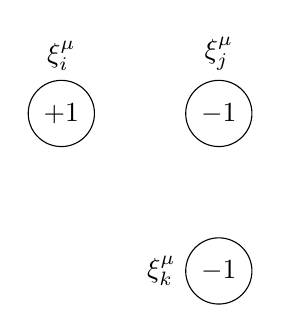
\begin{tikzpicture}[baseline=(current bounding box.center)]
\node[draw, circle, label={$\xi_i^\mu$}] (a) at (-1, 0) {$+1$}; 
\node[draw, circle, label={$\xi_j^\mu$}] (b) at (1, 0) {$-1$};
\node[draw, circle, label=left:{$\xi_k^\mu$}] (c) at (1, -2) {$-1$};
\end{tikzpicture}
$\quad \overset{\text{Hebb's rule}}{\longrightarrow} \quad$
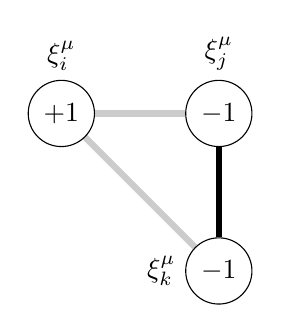
\begin{tikzpicture}[baseline=(current bounding box.center)]
\node[draw, circle, label={$\xi_i^\mu$}] (a) at (-1, 0) {$+1$}; 
\node[draw, circle, label={$\xi_j^\mu$}] (b) at (1, 0) {$-1$};
\node[draw, circle, label=left:{$\xi_k^\mu$}] (c) at (1, -2) {$-1$};

\draw[line width = 0.8mm, opacity = 0.2] (a) -- (b);
\draw[line width = 0.8mm, opacity = 0.2] (a) -- (c);
\draw[line width = 0.8mm, ] (c) -- (b);
\end{tikzpicture}
\end{document}